\documentclass[10pt]{article}
\usepackage[letterpaper,margin=1in]{geometry}
\usepackage[T1]{fontenc}
\usepackage{newtxtext,newtxmath}
\usepackage[protrusion=true,expansion=true]{microtype}
\usepackage{graphicx,booktabs,multirow,threeparttable,amsmath,enumitem,xcolor}
\usepackage[font=small,labelfont=bf,labelsep=period,skip=4pt]{caption}
\usepackage{tikz}
\usetikzlibrary{arrows.meta,positioning,fit,calc}
\usepackage[numbers,sort&compress]{natbib}
\usepackage[colorlinks=true,linkcolor=linkblue,citecolor=linkblue,urlcolor=linkblue]{hyperref}
\usepackage[capitalise,nameinlink]{cleveref}

\definecolor{linkblue}{HTML}{1F5FAE}
\definecolor{vblue}{HTML}{2A78D6}
\definecolor{vorange}{HTML}{EB6834}
\definecolor{vaqua}{HTML}{1BAF7A}
\definecolor{ink}{HTML}{0B0B0B}
\definecolor{ink2}{HTML}{52514E}
\definecolor{wash}{HTML}{F1F0EC}

\setlength{\parskip}{0.35em}
\setlength{\parindent}{0pt}
\setlist{itemsep=0.15em,topsep=0.3em,leftmargin=1.3em}
\renewcommand{\arraystretch}{1.12}
\newcommand{\x}{$\times$}

\title{\vspace{-1.2em}\textbf{Deduplicate, Don't Compress:}\\[0.15em]
\Large Storing and Serving Learned N-gram Memory}
\author{Yimin Du\\[0.2em]{\small \url{https://github.com/initial-d/ngram-store}}}
\date{\small November 2026}

\begin{document}
\maketitle

\begin{abstract}
\noindent Language models are acquiring large lookup memories: tables of learned vectors addressed by token n-grams, read sparsely at every step and kept in host memory at inference time.
We study three questions such a table raises, using controlled experiments on knowledge editing with frozen Qwen backbones, text classifiers with 7 and 34 million n-gram rows, and character n-gram embeddings.
\emph{When are distinct rows worth it?} Per-key rows beat hashed rows by 0.4--4.1 points on MultiCounterFact, more so as the number of stored facts grows, while for language-model perplexity a single constant per hash head recovers the branch's effect.
\emph{What does training leave behind?} With sum or mean pooling and sparse SGD, rows that occur in the same bags receive identical updates; on a zero-initialized AG News table, rows are byte-identical exactly when their bag incidence is identical, which makes 87\% of the table duplicates. Prefix/suffix neighbours of character n-grams also converge, from 3\% to 44\% mergeable rows as training lengthens.
\emph{How should the table be stored?} Block compression is the wrong tool for scattered lookups: one document decodes 16\,MiB of blocks to read 65\,KiB of rows. Storing only the distinct rows, uncompressed, keeps 85--86\% of the saving and serves the full GPU host path at 1.09--1.23\x{} the latency of raw memory, against 29--79\x{} for compressed layouts. NGramStore, an open-source engine, implements these layouts and a planner that predicts their sizes to the byte.
\end{abstract}

% ------------------------------------------------------------------
\section{Introduction}

Lookup memories are back in large models. Engram~\citep{deepseek2026engram} hashes token n-grams into embedding tables and gates the retrieved vectors into the residual stream; memory layers~\citep{lample2019large,berges2024memory}, over-tokenized input vocabularies~\citep{huang2025overtokenized} and n-gram embedding scaling~\citep{yu2025scone} follow the same pattern. The table grows with the vocabulary of keys rather than with compute, is touched by a handful of rows per token, and is frozen once training ends. In deployment it typically lives in host memory and is gathered on demand.

That makes the table a storage and serving problem, and an old one. FastText built word vectors from hashed character n-grams~\citep{bojanowski2017enriching}; recommendation systems serve embedding tables of billions of rows~\citep{naumov2019dlrm}. Two design choices recur. The first is \textbf{identity}: give every observed n-gram its own row, or hash keys into a fixed number of buckets~\citep{weinberger2009feature} and let unrelated keys share parameters. The second is the \textbf{storage layout} of the frozen table: dense, quantized, compressed, or deduplicated.

We study both with NGramStore, an engine for frozen n-gram tables, and with controlled experiments in which every number is tied to a frozen protocol, an archived result and, for most reports, a verifier script. Three findings organize the paper.

\begin{enumerate}[label=\arabic*.]
\item \textbf{Distinct rows are a capacity decision for per-key knowledge} (\cref{sec:identity}). On MultiCounterFact editing with frozen Qwen backbones, distinct rows beat matched hash buckets by 0.4--4.1 points of harmonic score at 20,877 edits, more than at 1,024 edits, and beat parameter-matched adapters by 5.4--7.0 points. For language-model perplexity, replacing every row of a trained branch by its head's mean changes test perplexity by 0.04\%.
\item \textbf{Training creates exact, predictable redundancy} (\cref{sec:redundancy}). Rows with identical bag incidence get identical gradients. On a 7-million-row AG News table with zero initialization, the partition of rows by incidence and the partition by bytes coincide, group for group; 87\% of rows are duplicates. Uniform initialization removes all of them. Prefix/suffix neighbours of character n-grams converge more slowly, from 3\% to 44\% mergeable rows between 2k and 32k steps.
\item \textbf{Deduplicate, don't compress} (\cref{sec:serving}). Block codecs make each scattered lookup decode a whole block. Keeping one uncompressed copy of each distinct row retains almost all of the saving and nearly all of the speed (\cref{fig:overview}b). The same holds for prefix/suffix sharing: 42.4\% of a 46.0\% saving at about 2\x{} raw lookup cost instead of 125\x.
\end{enumerate}

\begin{figure}[t]
\centering
\begin{minipage}[c]{0.44\linewidth}
\centering
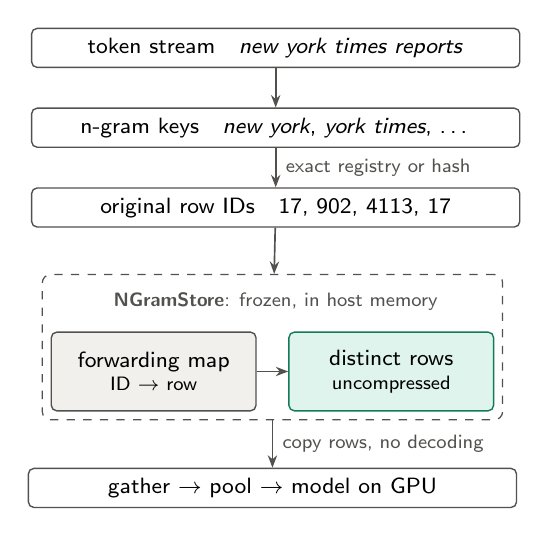
\begin{tikzpicture}[
  font=\sffamily\footnotesize, node distance=5mm,
  box/.style={draw=ink2, line width=0.5pt, rounded corners=2pt, fill=white, align=center, inner sep=3.5pt, minimum width=62mm},
  arr/.style={-{Stealth[length=4.5pt]}, line width=0.6pt, draw=ink2},
  lab/.style={font=\sffamily\scriptsize, text=ink2}]
\node[box] (tok) {token stream\quad \textit{new york times reports}};
\node[box, below=of tok] (keys) {n-gram keys\quad \textit{new york}, \textit{york times}, \dots};
\node[box, below=of keys] (ids) {original row IDs\quad 17, 902, 4113, 17};
\draw[arr] (tok) -- (keys);
\draw[arr] (keys) -- node[right, lab] {exact registry or hash} (ids);
\node[lab, below=7mm of ids] (storelab) {\textbf{NGramStore}: frozen, in host memory};
\node[box, below=1.5mm of storelab, xshift=-15.5mm, minimum width=26mm, minimum height=10mm, fill=wash] (map) {forwarding map\\[-1pt]{\scriptsize ID $\rightarrow$ row}};
\node[box, right=4mm of map, minimum width=26mm, minimum height=10mm, fill=vaqua!14, draw=vaqua!70!black] (rows) {distinct rows\\[-1pt]{\scriptsize uncompressed}};
\draw[arr] (map) -- (rows);
\node[draw=ink2, dashed, line width=0.45pt, rounded corners=3pt, fit=(storelab)(map)(rows), inner sep=3pt] (store) {};
\draw[arr] (ids) -- (store);
\node[box, below=6mm of store] (gpu) {gather $\rightarrow$ pool $\rightarrow$ model on GPU};
\draw[arr] (store) -- node[right, lab] {copy rows, no decoding} (gpu);
\end{tikzpicture}\\[0.2em]
{\small (a)}
\end{minipage}\hfill
\begin{minipage}[c]{0.54\linewidth}
\centering
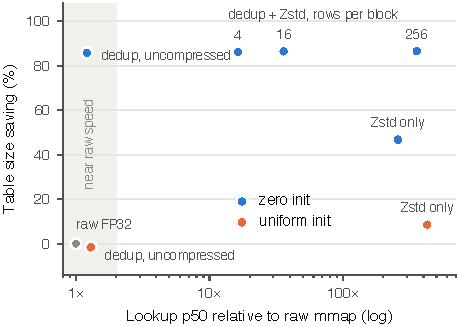
\includegraphics[width=\linewidth]{figures/tradeoff.pdf}\\[0.1em]
{\small (b)}
\end{minipage}
\caption{\textbf{(a)} Serving path for a learned n-gram table. A model maps n-grams to row IDs; the store forwards each ID to one of the distinct rows and copies it out. \textbf{(b)} Table saving against lookup latency for layouts of a trained 7-million-row AG News table (Apple M5, per-document lookups over the full test set). With zero initialization, deduplication alone gives 85.8\% at 1.2\x{} raw; adding Zstd gains 0.8 points and costs 16--356\x. With uniform initialization nothing is duplicated and compression saves 8.5\% at 427\x.}
\label{fig:overview}
\end{figure}

The engine, layouts and planner are released as NGramStore~0.5.0. Its origin is a 2017 FastText prototype that assigned exact trie identities to n-grams and compacted rows after training~\citep{du2025mefasttext}; the system and all measurements here are new.

% ------------------------------------------------------------------
\section{Setting}
\label{sec:setting}

\paragraph{Learned n-gram memory.} A model holds a table $E \in \mathbb{R}^{N\times d}$ and a map from n-gram keys to row IDs. With exact addressing each registered key owns a row; with hashing, $N$ is fixed and keys collide. The model reads rows either as bags pooled by sum or mean (FastText, our classifiers) or one row per hash head (Engram). At inference the table is frozen; a request gathers rows on the host and ships the pooled result or the rows to the accelerator.

\paragraph{NGramStore.} The engine stores a table as fixed-width rows grouped in blocks. Each block is stored raw or compressed (zlib, LZ4, Zstd~\citep{collet2021zstd}, optionally on XOR residuals of adjacent rows). An optional forwarding map sends original IDs to physical rows, which enables deduplication, reordering and representative sharing; without it, row $i$ is original ID $i$. Optional string keys are indexed with a double-array trie~\citep{aoe1989efficient}, which also exposes prefix and suffix chains, and shared rows are compacted as in a mark-compact collector~\citep{jones2011gc}. A C gather API, PyTorch adapters and a \texttt{plan} command (\cref{sec:planner}) sit on top. All lossless layouts return the stored bytes exactly.

\begin{table}[t]
\centering
\small
\caption{Workloads. All tables are 128-dimensional FP32 unless noted.}
\label{tab:workloads}
\begin{tabular}{@{}lllll@{}}
\toprule
Workload & Keys & Table & Model & Used in \\
\midrule
Knowledge editing & token n-grams, exact/hashed & per-edit rows & Qwen3-0.6B, Qwen3.5-4B~\citep{qwen3} & \S\ref{sec:identity} \\
Language modeling & token n-grams, hashed & TinyEngram branch~\citep{tinyengram} & Qwen3-0.6B & \S\ref{sec:identity} \\
AG News & word 1--4-grams, exact & 6.99M rows, 3.3\,GiB & mean bag + linear & \S\ref{sec:redundancy}, \S\ref{sec:serving} \\
DBpedia & word 1--4-grams, exact & 34.05M rows, 16.2\,GiB & mean bag + linear & \S\ref{sec:serving} \\
Character SGNS & char n-grams, order $\le$ 12 & 18,137 rows & skip-gram~\citep{mikolov2013distributed} & \S\ref{sec:redundancy}, \S\ref{sec:serving} \\
\bottomrule
\end{tabular}
\end{table}

\paragraph{Workloads.} \Cref{tab:workloads} lists them. Knowledge editing follows MultiCounterFact~\citep{meng2023memit}: an n-gram memory branch on a frozen Qwen backbone learns 1,024 or 20,877 counterfactual edits, scored by the harmonic mean $H$ of rewrite, paraphrase and neighbourhood success. The classifiers use the full official AG News and DBpedia splits~\citep{zhang2015character}, word 1--4-grams over complete documents, mean pooling and a linear head, trained with sparse SGD from zero or uniform initialization, three seeds each. The character model is skip-gram with subword bags on a 200k-token enwik8 prefix~\citep{mahoney2011enwik8}. Each experiment has a protocol fixed before the run; unless stated, intervals are paired 95\% bootstrap intervals over seeds and cases.

% ------------------------------------------------------------------
\section{When do distinct rows pay off?}
\label{sec:identity}

\begin{figure}[t]
\centering
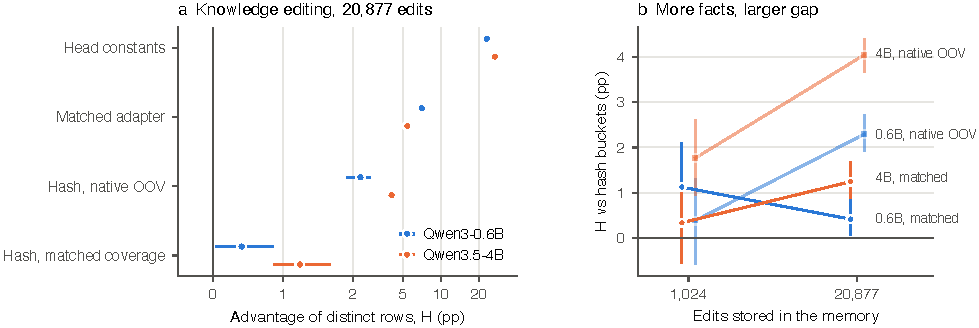
\includegraphics[width=\linewidth]{figures/identity.pdf}
\caption{Value of distinct n-gram rows on MultiCounterFact (frozen backbones, three seeds, 95\% intervals). \textbf{(a)} At 20,877 edits the full-key branch beats every independently trained control; the x-axis is linear below 2 and logarithmic above. \textbf{(b)} Against hash buckets of matched coverage (circles) and the native open-vocabulary hash contract (squares, faded), the gap is larger at 20,877 edits than at 1,024 in three of four comparisons.}
\label{fig:identity}
\end{figure}

\paragraph{Knowledge editing.} Exact and hashed memories are matched in row bytes, parameters, initial vectors and training exposures. At 20,877 edits the exact branch leads matched-coverage hashing by 0.41 [0.04, 0.86] points of $H$ on Qwen3-0.6B and 1.24 [0.87, 1.68] on Qwen3.5-4B, and leads the native open-vocabulary hash contract by 2.29 and 4.05 (\cref{fig:identity}a). Both models pass the preregistered gate against both hash controls: a positive $H$ interval with no neighbourhood regression beyond 2 points. Against independently trained alternatives with the same backbone and exposures, the full-key branch wins by 5.4--7.0 points over a parameter-matched adapter and by 23--27 points over one learned constant per hash head.

At 1,024 edits the picture is mixed: two of four hash comparisons have intervals crossing zero, and in a separate grid that varies table size, no larger table gives a stable gain and a BM25 retriever scores highest. The pattern in \cref{fig:identity}b is the one a capacity argument predicts. Collisions cost little when few keys carry information and more as the number of facts that must stay separable grows.

\paragraph{Language modeling.} A TinyEngram branch trained on Qwen3-0.6B lowers held-out perplexity: bypassing it raises test perplexity by 11.2\% [9.0, 13.6]. Replacing every row in each hash head by that head's mean raises it by only 0.04\% [$-$0.09, 0.18], with the backbone, gates and token IDs unchanged. In a follow-up that also trains the last two decoder layers, the full table loses to both an independently trained head-constant model and a memory-free model on all three seeds. For this objective the branch acts as a learned bias per head; per-key rows add nothing measurable.

\paragraph{Takeaway.} Distinct rows earn their memory when the task stores per-key facts and the number of facts approaches the capacity of the hashed table. A table that only shifts the model's output distribution can be replaced by constants. Both cases call for a necessity check, comparing the memory against memory-off, per-head constants and a matched adapter, before the table is scaled up.

% ------------------------------------------------------------------
\section{Training makes tables redundant}
\label{sec:redundancy}

\paragraph{Identical incidence, identical rows.} Let a model read row $e_i$ through bags $b$ with multiplicity $A_{bi}$, pooled by sum or mean. The gradient of the loss with respect to $e_i$ is $\sum_b A_{bi}\, w_b\, g_b$, where $g_b$ is the gradient at the pooled vector and $w_b$ the pooling weight. Two rows with the same incidence column, $A_{\cdot i} = A_{\cdot j}$, therefore receive the same gradient at every step, and under sparse SGD with a shared learning rate
\begin{equation}
e_i(t) - e_j(t) = e_i(0) - e_j(0).
\label{eq:incidence}
\end{equation}
With zero initialization, rows with identical incidence stay identical, and because they see the same floating-point operations in the same order, they stay \emph{byte}-identical. The converse is not implied: rows with different incidence could coincide by accident.

On the AG News table (6,989,611 trained rows, zero initialization, ten epochs), we grouped rows by their set of (document, multiplicity) pairs and, separately, by their bytes. Both partitions have exactly 883,125 groups, and their intersection has 883,125 groups too: rows are duplicates if and only if their incidence matches. Most of the effect comes from the long tail; 78.6\% of keys occur exactly once in training, and all once-seen n-grams of a document share one row value. \Cref{fig:redundancy}a shows the result on the controlled tables: 87.4\% of AG News rows and 86.5\% of DBpedia rows are duplicates under zero initialization and none under uniform initialization, exactly as \cref{eq:incidence} predicts, since distinct initial values never converge.

\begin{figure}[t]
\centering
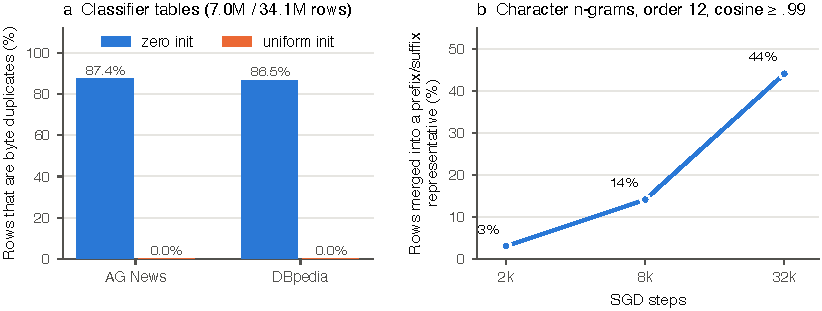
\includegraphics[width=\linewidth]{figures/redundancy.pdf}
\caption{Redundancy left by training. \textbf{(a)} Byte-duplicate rows in the controlled classifier tables (mean of three seeds). Zero initialization keeps rows with identical bag incidence identical; uniform initialization keeps them apart. \textbf{(b)} Character n-gram rows that join a prefix/suffix representative at cosine and norm ratio $\ge$ .99, for three seeds (thin) and their median, as training lengthens. The accumulated update grows from 10.6 to 32.8 times the initialization norm over the same range.}
\label{fig:redundancy}
\end{figure}

\paragraph{Prefix/suffix convergence.} Character n-grams that are prefixes or suffixes of one another share most of their incidence, so their updates are close but not identical. Over training the common update dominates the initialization and the rows converge in direction and norm. On the character skip-gram model (maximum order 12), the fraction of rows that pass a cosine and norm-ratio threshold of .99 against a trie neighbour grows from 3\% at 2k steps to 14\% at 8k and 44\% at 32k (\cref{fig:redundancy}b), while the ratio of accumulated update to initialization norm grows from 10.6 to 32.8. Merging those rows changes held-out skip-gram loss by less than $6\times10^{-5}$ relative on test and confirmation text. Longer training also raises the source model's held-out loss, so this describes what training does to the table's structure, not a recommended training length.

% ------------------------------------------------------------------
\section{Deduplicate, don't compress}
\label{sec:serving}

\paragraph{Why compression is slow here.} A block codec saves space only if a block holds many rows, and a lookup must decode the whole block to read one row. The classifier registry is sorted by key bytes, so the 130 rows of an average AG News document fall in different blocks. With the 256-row blocks used in the deployment grid, one document decodes up to $130 \times 128$\,KiB $= 16$\,MiB to return 65\,KiB. \Cref{fig:decode}a measures this directly: per-document latency falls in proportion to block size, from 5.1\,ms at 256 rows to 0.23\,ms at 4 rows, and is still 16\x{} raw at the smallest block that compresses at all. Batching documents helps only where they share blocks; 32 documents per call reduce total time 1.25--1.6\x.

\begin{figure}[t]
\centering
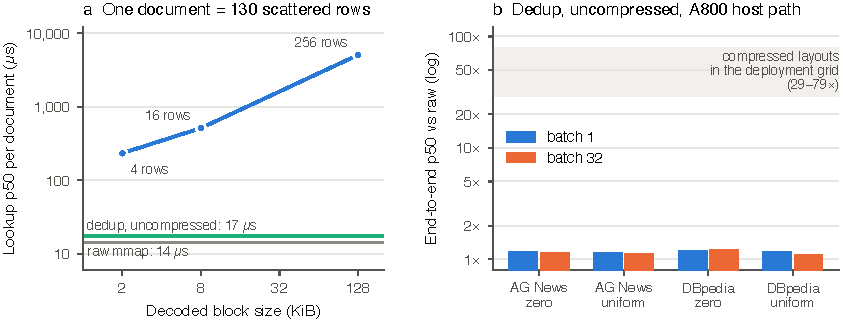
\includegraphics[width=\linewidth]{figures/decode.pdf}
\caption{Cost of decoding on scattered lookups. \textbf{(a)} Per-document p50 on the zero-initialized AG News table against decoded block size, with the uncompressed deduplicated layout and raw memory for reference (Apple M5). \textbf{(b)} The complete GPU host path of the deployment grid, using its own staging code and request set, with the uncompressed deduplicated layout. Bars are p50 relative to raw memory on the same A800; the shaded band is the range the grid reported for the compressed layouts it selected. Logits are byte-identical to raw in every case.}
\label{fig:decode}
\end{figure}

\paragraph{Keep the distinct rows, uncompressed.} Deduplication stores each distinct row once and forwards original IDs to it with an 8-byte map entry. A lookup then copies rows; nothing is decoded. On the zero-initialized tables this layout saves almost as much as the compressed one, because the compressible content \emph{was} the duplicates (\cref{tab:serving}). On all twelve original tables of the deployment grid it saves 85.0--85.8\%, against 85.7--86.6\% for deduplication plus Zstd, and CPU lookups run at 1.4--1.9\x{} raw memory. Through the grid's complete GPU host path, with its own request set, staging and reductions, the end-to-end latency is 1.09--1.23\x{} raw, where the selected compressed layouts measured 29--79\x{} (\cref{fig:decode}b). Logits are byte-identical. Passing NumPy buffers straight to the C gather matters at this point: once decoding is gone, building a Python list of IDs per call doubles lookup time.

\begin{table}[t]
\centering
\small
\caption{Layouts on the twelve original deployment-grid tables (three seeds per row). Saving is relative to the FP32 table file. CPU lookup is per document over 5,000 test documents; GPU path is batch 1 / batch 32 for seed 3, relative to raw memory.}
\label{tab:serving}
\begin{tabular}{@{}llrrrrl@{}}
\toprule
& & \multicolumn{2}{c}{Saving} & \multicolumn{2}{c}{Dedup, uncompressed} & \\
\cmidrule(lr){3-4}\cmidrule(lr){5-6}
Dataset & Init & Grid selection & Dedup, uncompressed & CPU lookup & GPU path & Planner \\
\midrule
AG News & zero & 86.58--86.59\% & 85.80\% & 1.74--1.76\x & 1.18 / 1.14\x & dedup \\
DBpedia & zero & 85.68--85.69\% & 84.95\% & 1.44--1.77\x & 1.19 / 1.23\x & dedup \\
AG News & uniform & 8.54--8.55\% & $-$1.59\% & 1.81--1.87\x & 1.16 / 1.14\x & raw \\
DBpedia & uniform & 8.87--8.88\% & $-$1.59\% & 1.85--1.88\x & 1.18 / 1.09\x & raw \\
\bottomrule
\end{tabular}
\end{table}

On the uniform tables there is nothing to deduplicate: the map costs 1.6\% and compression saves 8.5--8.9\%. A layout that saves 9\% at 400\x{} the lookup cost is rarely the right trade, and the planner keeps such tables raw.

\paragraph{Structure stored the same way.} Prefix/suffix sharing merges a row into its representative, which makes the two byte-identical, so the merged table can use the same layout. On the nine character-model checkpoints of \cref{fig:redundancy}b, the uncompressed deduplicated form saves 1.5\%, 12.6\% and 42.4\% at 2k, 8k and 32k steps, against 7.2\%, 18.0\% and 46.0\% for the original XOR-plus-zlib blocks, and lookups run at about 2\x{} raw instead of about 125\x. Every decoded row matches the shared table byte for byte.

\paragraph{Choosing a layout.}
\label{sec:planner}
\texttt{ngram-store plan} hashes every row, counts distinct rows and computes the exact size of the raw and deduplicated uncompressed layouts, recommending the smaller; with \texttt{-{}-prefer size} it also estimates compressed layouts from 64 sampled blocks. On the twelve grid tables its uncompressed sizes equal the packed files byte for byte, its compressed estimates are within 0.15\%, and with \texttt{-{}-prefer size} it picks the same codec family as the grid's calibration on all twelve. A 3.5\,GB table takes about five seconds on a laptop.

% ------------------------------------------------------------------
\section{Related work}

\paragraph{Hashed and compressed embeddings.} The hashing trick~\citep{weinberger2009feature} and FastText's bucketed subwords~\citep{bojanowski2017enriching,joulin2017bag} bound table size by sharing rows across keys; compositional~\citep{shi2020compositional} and tensor-train~\citep{yin2021ttrec} embeddings factor the table instead. Quantization and product quantization~\citep{jegou2011product,johnson2019billion} compress rows lossily. These methods change the vectors; the layouts here keep them and exploit exact redundancy that the training procedure creates.

\paragraph{Lookup memory in language models.} Product-key memories~\citep{lample2019large} and memory layers at scale~\citep{berges2024memory} add large sparse tables to transformers; over-tokenized vocabularies~\citep{huang2025overtokenized}, SCONE~\citep{yu2025scone} and Engram~\citep{deepseek2026engram} attach n-gram embeddings, with Engram reading hashed n-grams per head into the residual stream. Non-parametric n-gram models such as infini-gram~\citep{liu2024infinigram} index counts rather than learned vectors. Our results bear on the tables these designs produce: when exact keys are worth their rows, what redundancy training leaves in them, and how to serve them from host memory.

\paragraph{Embedding serving.} Recommendation systems~\citep{naumov2019dlrm} face the same sparse-gather pattern at larger scale and rely on caching, sharding and quantization. Our finding that decode amplification, not bandwidth, dominates compressed lookups applies to any block-compressed embedding store.

% ------------------------------------------------------------------
\section{Limitations}

The identity results come from one editing benchmark and one small language-model branch, with frozen or partly frozen backbones; they do not address Engram-style pretraining at scale. The redundancy mechanism is exact for sum or mean pooling with plain sparse SGD and a shared learning rate; adaptive optimizers with per-row state, dropout on rows, or per-row learning rates break \cref{eq:incidence}, and how much duplication survives them is untested. The serving measurements use single-node host gathers without row caching across requests; tables with strong request locality favour caches and can change the trade-off, as our cached Qwen traces showed. The structure-sharing lookups use random bags on a cache-resident table, so their ratios show decoding cost rather than large-table behaviour.

% ------------------------------------------------------------------
\section{Conclusion}

Learned n-gram tables are worth their rows when a task stores per-key facts at a scale where hashing collides, and are often redundant in exactly the way the training procedure dictates: identical incidence produces identical rows, and shared prefixes pull rows together over time. Serving such a table is a matter of indexing that redundancy, not entropy-coding it. Keeping one uncompressed copy of each distinct row, and keeping tables without duplicates raw, preserves nearly all of the space saving at close to raw lookup speed. For new lookup-memory designs this suggests two cheap habits: run a necessity check against per-head constants before scaling the table, and choose the initialization with the serving layout in mind.

\paragraph{Reproducibility.} NGramStore 0.5.0, all protocols, archived results and verifier scripts are at \url{https://github.com/initial-d/ngram-store}; every number in this report links to a directory under \texttt{evidence/}, and the figures are generated from those files by \texttt{docs/report/make\_figures.py}.

\small
\bibliographystyle{plainnat}
\bibliography{refs}

\end{document}
